%%% Hlavní soubor. Zde se definují základní parametry a odkazuje se na ostatní části. %%%

%% Verze pro jednostranný tisk:
% Okraje: levý 40mm, pravý 25mm, horní a dolní 25mm
% (ale pozor, LaTeX si sám přidává 1in)
\documentclass[12pt,a4paper]{report}
\setlength\textwidth{145mm}
\setlength\textheight{247mm}
\setlength\oddsidemargin{15mm}
\setlength\evensidemargin{15mm}
\setlength\topmargin{0mm}
\setlength\headsep{0mm}
\setlength\headheight{0mm}
% \openright zařídí, aby následující text začínal na pravé straně knihy
\let\openright=\clearpage

%% Pokud tiskneme oboustranně:
% \documentclass[12pt,a4paper,twoside,openright]{report}
% \setlength\textwidth{145mm}
% \setlength\textheight{247mm}
% \setlength\oddsidemargin{14.2mm}
% \setlength\evensidemargin{0mm}
% \setlength\topmargin{0mm}
% \setlength\headsep{0mm}
% \setlength\headheight{0mm}
% \let\openright=\cleardoublepage

%% Vytváříme PDF/A-2u
\usepackage[a-2u]{pdfx}

%% Přepneme na českou sazbu a fonty Latin Modern
\usepackage[czech]{babel}
\usepackage{lmodern}
\usepackage[T1]{fontenc}
\usepackage{textcomp}

%% Použité kódování znaků: obvykle latin2, cp1250 nebo utf8:
\usepackage[utf8]{inputenc}

%%% Další užitečné balíčky (jsou součástí běžných distribucí LaTeXu)
\usepackage{amsmath}        % rozšíření pro sazbu matematiky
\usepackage{amsfonts}       % matematické fonty
\usepackage{amsthm}         % sazba vět, definic apod.
\usepackage{bbding}         % balíček s nejrůznějšími symboly
			    % (čtverečky, hvězdičky, tužtičky, nůžtičky, ...)
\usepackage{bm}             % tučné symboly (příkaz \bm)
\usepackage{graphicx}       % vkládání obrázků
\usepackage{fancyvrb}       % vylepšené prostředí pro strojové písmo
\usepackage{indentfirst}    % zavede odsazení 1. odstavce kapitoly
\usepackage{natbib}         % zajištuje možnost odkazovat na literaturu
			    % stylem AUTOR (ROK), resp. AUTOR [ČÍSLO]
\usepackage[nottoc]{tocbibind} % zajistí přidání seznamu literatury,
                            % obrázků a tabulek do obsahu
\usepackage{icomma}         % inteligetní čárka v matematickém módu
\usepackage{dcolumn}        % lepší zarovnání sloupců v tabulkách
\usepackage{booktabs}       % lepší vodorovné linky v tabulkách
\usepackage{paralist}       % lepší enumerate a itemize
\usepackage{colortbl}			%tabulka
\usepackage[usenames]{xcolor}  % barevná sazba

%%% Údaje o práci

% Název práce v jazyce práce (přesně podle zadání)
\def\NazevPrace{Varianty Eberhardovy věty}

% Název práce v angličtině
\def\NazevPraceEN{Eberhard-Like Theorems}

% Jméno autora
\def\AutorPrace{Zuzana Šimečková}

% Rok odevzdání
\def\RokOdevzdani{2018}

% Název katedry nebo ústavu, kde byla práce oficiálně zadána
% (dle Organizační struktury MFF UK, případně plný název pracoviště mimo MFF)
\def\Katedra{Informatický ústav Univerzity Karlovy}
\def\KatedraEN{Computer Science Institute of~Charles University}

% Jedná se o katedru (department) nebo o ústav (institute)?
\def\TypPracoviste{Ústav}
\def\TypPracovisteEN{Institute}

% Vedoucí práce: Jméno a příjmení s~tituly
\def\Vedouci{doc. Mgr. Robert Šámal, Ph.D.}

% Pracoviště vedoucího (opět dle Organizační struktury MFF)
\def\KatedraVedouciho{Informatický ústav Univerzity Karlovy}
\def\KatedraVedoucihoEN{Computer Science Institute of~Charles University}

% Studijní program a obor
\def\StudijniProgram{Informatika}
\def\StudijniObor{IOI}

% Nepovinné poděkování (vedoucímu práce, konzultantovi, tomu, kdo
% zapůjčil software, literaturu apod.)
\def\Podekovani{%
Děkuji doc. Mgr. Robertu Šámalovi, Ph.D., vedoucímu práce, za ochotu, trpělivost, odborné rady a čas, které mi věnoval. Za výběr tématu a připomínky při řešení i sepisování práce.
}

% Abstrakt (doporučený rozsah cca 80-200 slov; nejedná se o zadání práce)
\def\Abstrakt{%
Pro konkrétní nakreslení rovinného grafu definujme posloupnost $(p_k)=(p_3,p_4,\dots)$ počtu stěn velikosti $k$ -- $k$-úhelníků. Z důsledku Eulerova vzorce o rovinných grafech pro kubické grafy splňuje $p$ vztah $\sum_{k \geq 3}{(6-k)p_k}=12$. Je celkem přirozené ptát se, jak vypadají $p$, pro které existuje odpovídající graf. Eberhard ukázal, že pokud $p$ vyhovuje důsledku Eulerova vzorce, pak existuje rovinný kubický graf, který odpovídá $p$ až na počet šestiúhelníků. VaMos a kol. dokázali obdobu věty, kde je povoleno k $p$ přidat pětiúhelníky a sedmiúhelníky. V této práci na jejich výsledky navazujeme, využijeme jejich důkazové strategie a díky navrženému programu najdeme stavební bloky, které autorům k zobecnění věty chyběly. Výsledkem práce je následující věta: pro každou posloupnost $p$ nezáporných celých čísel splňující důsledek Eulerova vzorce existuje nekonečně mnoho kubických rovinných grafů, které $p$ odpovídají až na $r$-úhelníky a $s$-úhelníky, pro každou z dvojic splňující $r,s \in \mathbb{N}, s<6<r<14 $ a $ s$, $r$ jsou nesoudělné.
}
\def\AbstraktEN{%
Abstract.
}

% 3 až 5 klíčových slov (doporučeno), každé uzavřeno ve složených závorkách
\def\KlicovaSlova{%
{kubické grafy} {rovinné grafy} {Eberhardova věta} {kreslení grafů} 
}
\def\KlicovaSlovaEN{%
{cubic graphs} {planar graphs} {Eberhard's theorem} {graph drawing}
}

%% Balíček hyperref, kterým jdou vyrábět klikací odkazy v PDF,
%% ale hlavně ho používáme k uložení metadat do PDF (včetně obsahu).
%% Většinu nastavítek přednastaví balíček pdfx.
\hypersetup{unicode}
\hypersetup{breaklinks=true}

%% Definice různých užitečných maker (viz popis uvnitř souboru)
\include{makra}

%% Titulní strana a různé povinné informační strany
\begin{document}
\include{titulka}

%%% Strana s automaticky generovaným obsahem bakalářské práce

\tableofcontents

%%% Jednotlivé kapitoly práce jsou pro přehlednost uloženy v samostatných souborech
\chapter*{Úvod}
\addcontentsline{toc}{chapter}{Úvod}

Zkusíme-li upravovat Eulerův vzorec pro rovinné grafy
$|V|-|E|+|S|=2$, můžeme pro kubické grafy dospět do tvaru 
\begin{equation}\label{eq01:neccCond}
\sum_{k \geq 3}{(6-k)p_k}=12,
\end{equation}
kde $p_k$ značí počet $k$-hranných stěn grafu. Výraz \eqref{eq01:neccCond} je nutnou podmínkou pro rovinnost kubického grafu. Pozoruhodně, počet šestihranných stěn v této podmínce nehraje žádnou roli. Toho si všiml Victor Eberhard a v roce 1981 formuloval a dokázal, že pokud můžeme volit $p_6$, dokážeme najít graf zadaný počtem ostatních stěn, který je rovinný.

Abychom mohli větu formulovat formálně, je nutné definovat přijatelné posloupnosti: posloupnost $(p_k) = (p_3,p_4,...)$ kladných celých čísel je přijatelná, pokud existuje rovinný kubický 3-spojitý graf, který má právě $p_k$ $k$-hranných stěn.

Přidáním podmínky na 3-spojitost získáváme jen grafy, které (podle Steinitzovy věty) odpovídají konvexním 3-polytopům. Ekvivalentně lze tedy přijatelnou posloupnost definovat následovně:

\begin{definice}[Přijatelná posloupnost]\label{def01:1}
Posloupnost $(p_k) = (p_3,p_4,...)$ kladných celých čísel je přijatelná, pokud existuje jednoduchý (vrcholy mají stupeň 3) 3-polytop, který má právě $p_k$ $k$-hranných stěn.
\end{definice}

Formulujme nyní Eberhardovu větu //TODO odkaz:
\begin{veta}[Eberhardova věta]\label{veta01:1}
Pro každou posloupnost $(p_k | 3 \leq k \neq 6)$ kladných celých čísel, splňující \eqref{eq01:neccCond} existuje taková hodnota $p_6$, že $(p_k | k\geq 3)$ je přijatelná.
\end{veta}

%%% Fiktivní kapitola s ukázkami sazby

\chapter{Pojmy a definice}

\section{sekce 1}
Definice: 

TODO zmínit, že o triarku často budeme mluvit jako o trojúhelníku (rovnorammený, základna...)

TODO řešítko neumí udržovat poměry stěn z neutrální posloupnosti

TODO zavést, že z posloupnost x získáme množinu velikostí stěn, které jsou v x nenulové jako X

\chapter{Konstrukce důkazu}

Představme hypotézu, kterou se snažíme ověřit.
\begin{hypot}\label{veta02:hypoteza}
Mějme přípustnou posloupnost $p=(p_k | 3 \leq k \neq 6)$ a neutrální posloupnost $q=(q_k \mid 3 \leq k \neq 6)$, pak existuje takové přirozené $n$, že $p+nq$ je přijatelná.
\end{hypot}

TODO zmínit výjimku pro torus.

V článku \citep{Samal09} autoři naznačují konstrukci důkazu, za předpokladu, že existují nějaké pomocné grafy. V další kapitole představíme způsob, jak takové grafy hledat. Teď se zaměříme na důkaz samotný, respektive nejprve představíme graf, který v důkazu pomáhal již Eberhardovi.

\section{Triarky a operace s nimi}

\begin{definice}[Triark]\label{def02:1}
Triark je takový rovinný graf $T$, že vrcholy jeho vnější stěny tvoří cyklus $C$, každý vnitřní vrchol (tj. vrcholy $T-C$) má v $T$ stupeň právě 3 a v $C$ jsou tři navzájem různé vrcholy $x$, $y$, $z$ stupně 2 - \textbf{rohy}, že vrcholy každé ze tří cest v C, které vzniknou odstraněním rohů z C, mají střídavě stupeň 2 a 3, počínaje i konče stupněm 2.
\end{definice}

\textbf{Strana} triarku je každá z výše zmíněných cest v C, ke které na oba konce připojíme i příslušný roh. \textbf{Délka strany} triarku odpovídá počtu jejích vnitřních vrcholů stupně 2 v T. O triarku se stranami délky $a$, $b$, $c$ mluvíme jako o ($a$, $b$, $c$,)-\textbf{triarku}. Poznamenejme, že na pořadí stran v názvu nezáleží (odpovídají rotacím). Později využijeme ještě dalšího značení. $M$-\textbf{triark} má vnitřní strany pouze velikostí z $M$. U triarku přejímáme některé termíny používané pro trojúhelníky a jejich význam bude vždy intuitivní.

\begin{figure}[h!]\centering
\includegraphics[height=60mm]{../img/triarc}
\caption{Ukázka (4,4,3)$ \lbrace 4,7\rbrace $-triarku.}
\label{obr03:triark}
\end{figure}

Zmiňme velmi užitečnou vlastnost triarků: pokud máme dva triarky, oba mající stranu stejné délky, můžeme je za tuto stranu slepit a získáme opět graf, jehož vnitřní vrcholy mají stupeň 3. (Při slepovaní se ztotožní vždy vrchol stupně 2 s vrcholem stupně 3.) Pokud slepíme triarky tak, že protější strany výsledného grafu budou stejně dlouhé (tedy speciálně při slepení dvou stejný triarků), budeme podle jeho tvaru mluvit o \textbf{rovnoběžníku}. Rovnoběžníky jdou navíc slepovat podobně jako triarky a můžeme tím každý již existující rovnoběžník zvětšit na libovolný rozměr, který je násobkem jeho původních rozměrů.


\begin{figure}[h!]\centering
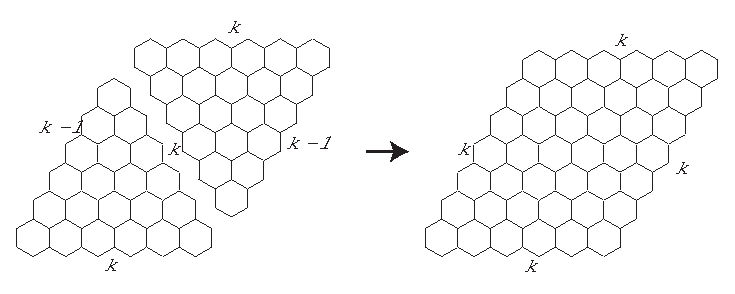
\includegraphics[width=\textwidth]{../img/T-P}
\caption{Spojení dvou triarků za vzniku rovnoběžníku.}
\label{obr21:T-P}
\end{figure}

Mohli bychom ale chtít spojovat triarky tak, aby výsledkem byl opět triark. Mějme ($a_1$, $b_1$, $c_1$)-triark a ($a_2$, $b_2$, $c_2$)-triark a vhodný rovnoběžník. Slepením, jako na obrázku \ref{obr22:T-T}, vznikne ($a_1+a_2$, $b_1+b_2$, $c_1+c_2$)-triark. 

\begin{figure}[h!]\centering
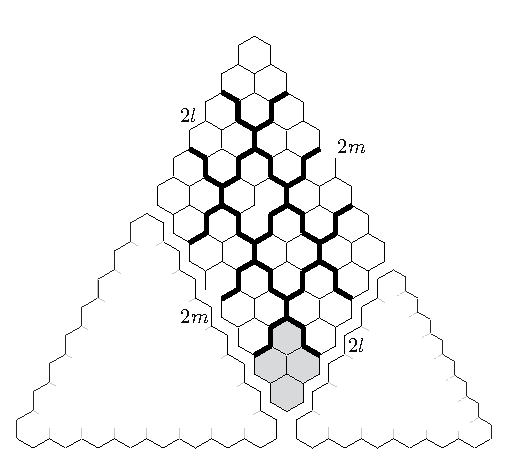
\includegraphics[width=\textwidth]{../img/T-T}
\caption{Spojení triarků spolu s rovnoběžníkem za vzniku triarku.}
\label{obr22:T-T}
\end{figure}

A závěrem budeme chtít spojit dva triarky tak, aby výsledkem byl kubický graf (tedy aby nevznikly žádné nové stěny s vrcholy stupně dva). Graf, který má tuto funkci označíme za \textbf{prstenec}. Jde o souvislý graf, ve kterém můžeme vyznačit dva disjunktní cykly tak, že stupně vrcholů každého cyklu jsou opačné než stupně příslušných triarků, které chceme spojit. Kde opačně znamená záměna dvoj- a tří- vaznosti vrcholů. Způsob spojení odpovídá přesně zavedení definice, ale je znázorněno i na obrázku \ref{obr23:T-G}. 

\begin{figure}[h!]\centering
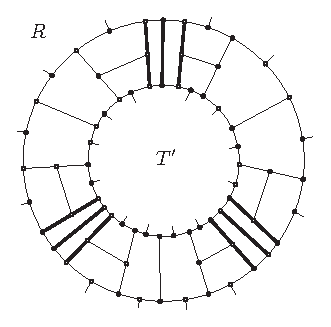
\includegraphics[height=40mm]{../img/T-G}
\caption{Spojení triarků prstencem za vzniku kubického grafu.}
\label{obr23:T-G}
\end{figure}

TODO připravit vlastní obrázky (které víc odpovídají popiskům) pro ukázku slepování.


\section{Důkaz za předpokladu existence pomocných grafů}
Převeďme hypotézu ve větu.

\begin{veta}\label{veta02:2}
Mějme přípustnou posloupnost $p=(p_k | 3 \leq k \neq 6)$ a neutrální posloupnost $q=(q_k \mid 3 \leq k \neq 6)$ a následující grafy pro nějaké přirozené k:
\begin{description}
\item[(i)] ($k$, $k$, $k$),$Q$-triark;
\item[(ii)] ($k$, $k$, $k-1$),$Q$-triark;
\item[(iii)] rovnoramenný $Q\cup \lbrace1\rbrace$-triark, délky jehož stejných stran jsou dělitelné $k$ a který obsahuje právě jednu stěnu velikosti $l$ pro každé nenulové $p_l$ v $p$, této stěně říkejme \textbf{jádro} triarku;
\item[(iv)] prstenec, který dokáže spojit dva stejně velké, rovnostranné triarky.
\end{description}

Pak existuje takové přirozené $n$, že $p+nq$ je přijatelná.
\end{veta}


Myšlenka důkazu pak není příliš složitá: každou stěnu ze zadané posloupnosti $p$ zabalíme do triarku (iii), připravíme si pomocné lepící a zkrášlující prvky (ii), díky kterým získáme jediný velký rovnostranný triark. K němu zkonstruujeme ještě jeden se stejně dlouhými (i) a pomocným prstencem je spojíme v kýžený graf (iv). Všechny tyto pomocné objekty jsou totiž (kromě jader) jen ze stěn, které jsou v zadané neutrální posloupnosti, lepicí operace zachovávají kubičnost uvnitř grafu a prstenec pak spojí dva triarky v hledaný kubický graf.

\textit{Důkaz.} Nejprve slepíme dva ($k$, $k$, $k-1$)-triarky za stěnu délky $k$ a získáme rovnoběžník se všemi stranami délky $k$. A díky slepování můžeme získat i libovolný rovnoběžník o rozměrech $mk$, $lk$ pro $m$, $l$ přirozená. Poté postupně spojujeme jednotlivé jádrové triarky za pomoci příslušného lichoběžníku, dokud nezískáme jediný triark, který obsahuje všechny stěny z $P$.

Zkusme vzniklý triark upravit na rovnostranný. Při slepování triarků se velikosti výsledných stran rovnají součtům původním. Pokud tedy slepujeme s ($k$, $k$, $k-1$)-triarkem, zmenšíme vždy tu stěnu, na kterou připadne rozměr $k-1$, vůči ostatním. Takže pokud budeme opakovat lepení výsledného triarku, v každém kroku se součet rozdílů mezi stranami zmenší a tedy nutně získáme rovnostranný triark. Modifikujme ho stejnou operací, aby zůstal rovnostranný, ale navíc délka jeho stran byla násobkem $k$ a označme výsledný triark $T_1$.

Slepováním ($k$,$k$,$k$)-triarků z (i) spolu s $k$,$k$ rovnoběžníky získáme druhý triark $T_2$ o stejném rozměru jako $T_1$. Kdybychom celý problém řešili na tóru, stačilo by $T_1$ a $T_2$ spojit do rovnoběžníku a sjednotit odpovídající strany. Na kouli místo toho použijeme prstenec z (iv). Tím získáme graf, který je kubický, rovinný a obsahuje požadované stěny.

TODO Možná poznamenat, že tím v podstatě je dokázána i verze věty, kde poslední řádek zní Pak existuje nekonečně mnoho takových přirozených $n$, že $p+nq$ je přijatelná.
%%% Fiktivní kapitola s ukázkami tabulek, obrázků a kódu

\chapter{Řešítko}
Abychom mohli dokončit důkaz některých instancí hypotézy \ref{veta02:hypoteza}, potřebujeme získat požadované stavební bloky. Nabízí se naprogramovat řešítko, které bude umět alespoň některé typy hledaných grafů najít. Hlavním cílem této práce bylo takový program připravit a pomocí něj získat lepší představu o potenciálu uvedené konstrukce důkazu.

\section{Algoritmus}

Program na vstupu očekává zadání vnější stěny: každý vrchol je zastoupen jedním bitem, který určuje, zda má být ve výsledném grafu stupně 2 nebo 3. Navíc očekává seznam velikostí stěn, které má využít. Na výstupu informuje, zda se mu daný graf podařilo najít (říkejme \textbf{vyplnit}), a umožní jej exportovat.

Postup hledání původně imitoval lidské pokusy o řešení problému: nakreslit si vnější stěnu, zkusit spojit nějaké dva vrcholy řetízkem vhodné délky (aby nově uzavřená stěna byla z neutrální posloupnosti) a dokud je místo na papíře, spojovat. Pak si překreslit nejvnitřnější, zatím neuzavřenou stěnu (budeme mluvit o \textbf{hranici}), ta se stane \uv{vnější stěnou} na novém papíře a pokračovat. V situaci, kdy nelze dál nic spojit, nebo je jasné, že graf nemůže vyhovovat parametrům, vrátit se podle uvážení zpět. Viz obrázek TODO odkaz.

Kdybychom chtěli znát jen ano/ne odpověď, jestli graf existuje, nebylo by vůbec třeba si pamatovat celý rozpracovaný graf, stačilo-by pracovat s hranicemi, které navíc stačí reprezentovat jako binární číslo. Výsledkem by pak mohla být jen posloupnost hranic, kterými se prošlo před uzavřením grafu, nebo samotné \uv{ano/ne}. Překvapivě obtížné je pak z této posloupnosti nestrojově získat skutečný graf, proto program nabízí i možnost graf dodatečně rekonstruovat podle prošlých stavů.

V tento okamžik je jasné, že problém je vlastně prohledávání v binárních řetězcích (které reprezentují hranice). Je proto vhodné zmínit, podle jakého kritéria se program rozhoduje, kterým směrem hledat dále. Implementace vždy upřednostňuje ke zpracování již nalezený řetězec nejmenší délky, a pro něj najde všechny další sousedy.

Aby toto prohledávání fungovalo dobře, je třeba trochu zkomplikovat reprezentaci hranice. Hlavním požadavkem bude identita mezi reprezentací (jediným binárním řetězcem) a všemi hranicemi (tedy cykly, na kterých vyznačené vrcholy ještě vyžadují dalšího souseda), které jsou pro algoritmus izomorfní - tedy všechny rotace a převrácení hranice.

\begin{definice}[Hranice a její reprezentace]\label{def01:1}
Cyklus $C$ a množinu $I \subseteq C(V)$ zveme hranicí $H$. Množina $I$ jsou právě ty vrcholy, které ve výsledném vyplnění musí mít dalšího souseda. Pokud  $i = \emptyset$, mluvíme o hranici přímo jako o stěně.

Binární řetězec (číslo) reprezentující hranici $H$ získáme následně: každý vrchol H označíme buď znakem 1 (jako I v "in" podle orientace pomyslené hrany) nebo 0 (jako 0 v "out"). Zaznamenejme pak všechny řetězce, které získáme čtením od každého vrcholu pro i proti směru hodinových ručiček. Ten z nich, který z nich má největší hodnotu (pokud řetězec chápeme jako binární číslo), je reprezentací hranice. Pokud $i = \emptyset$, pak přidejme speciální znak a zapamatujme počet vrcholů.
\end{definice}

Pro lepší představu přikládáme posloupnost hranic s vizualizací na obrázku \ref{obr03:reseni}, která řeší (4,4,3)$\lbrace$4,7$\rbrace$-triark. 

\begin{figure}[h!]\centering
\includegraphics[width=\textwidth]{../img/reseni}
\caption{Možný postup vyplnění (4,4,3)$\lbrace$4,7$\rbrace$-triarku. Hodnota pod grafem vždy odpovídá reprezentaci aktuální, tučně zvýrazněné, hranice.}
\label{obr03:reseni}
\end{figure}

Pro jistotu poznamenejme, že pokud program hledaný graf nenašel, může, ale nemusí to znamenat, že neexistuje.

Podle předchozí kapitoly pro dokončení důkazu pro konkrétní dvojici $p$ a $q$ a nějaké přirozené $k$ potřebujeme tyto čtyři typy grafů:
\begin{description}
\item[(i)] ($k$, $k$, $k$),$Q$-triark;
\item[(ii)] ($k$, $k$, $k-1$),$Q$-triark;
\item[(iii)] ($mk$,$mk$,$x$),$Q\cup \lbrace 1\rbrace$-triark, kde je právě jedna stěna velikosti $l$;
\item[(iv)] prstenec, který dokáže spojit dva stejně velké, rovnostranné triarky.
\end{description}

Pro dané $k$ získáme grafy (i) a (ii) z řešítka hned. Pro zbylé je nutné pomoci si konstrukcí, která se ukázala jako úspěšná pro některé neutrální sekvence. O výsledcích získaných z programu píšeme v další kapitole. TODO odkaz?

Na graf (iii) se neumíme zeptat přímo, protože potřebujeme v grafu mít právě jednu stěnu délky $p_l$. Spojme proto stěnu s vnější stěnou triarku ručně a ptejme se na výplň vzniklých oblastí $A$ a $B$. Ke spojení použijeme $l$ kopií řetízku $R$, každý napojíme na jeden z vrcholů jádra a druhé konce spojíme s \uv{in} vrcholy základny triarku. V řetízku navíc fixujeme, ve které straně od něj budou mít které jeho vrcholy třetího souseda (znázorněno šedě v obrázku TODO odkaz). Konstrukce je obecná pro všechny přípustné hodnoty $l$, tedy není závislá na volbě $p$. Navíc není (při dobré volně R) vynucená ani příliš velká stěna, takže konstrukce může být obecná i pro všechny q (protože q je neutrální, tedy v ní musí být nenulová hodnota na pozici reprezentující stěnu velikosti alespoň 6, tvrzení \eqref{veta:posloupnosti}.



Podobnou konstrukci tvoříme i pro graf typu (iv). V tomto případě za pomoci řetízků spojujeme odpovídající vrcholy rovnostranných, stejně velkých triarků $T_1$ a $T_2$. Vzniknou dva typy oblastí - $C$ při rozích triarku a $D$ mezi odpovídajícími kusy stran triarků. Poznamenejme, že na obrázku je $T_2$ nakreslen "naruby" TODO lepší slovo?. 

Tyto konstrukce jsou v řešítku implementovány. Výsledný program tedy na vstupu očekává seznam velikostí stěn, které mohou tvořit neutrální posloupnost. Pokud pro daný seznam stěn existuje více neutrálních posloupností, využije program pro každý pomocný graf libovolnou z nich.

\begin{figure}[h!]\centering
\includegraphics[width = \textwidth]{../img/iii+iv-construction}
\caption{Vlevo konstrukce grafu typu (iii), konkrétně ($xk$,$xk$,$l+1$)-triarku s jádrem velikosti $l$, vpravo konstrukce grafu typu (iv).}
\label{obr03:konstrukce}

\end{figure}

\section{Uživatelská dokumentace}



%%% Fiktivní kapitola s instrukcemi k PDF/A

\chapter{Výsledky}

Díky programu popsanému v předchozí kapitole bylo možné zkusit dokončit důkaz věty \eqref{veta02:hypoteza} pro některé neutrální posloupnosti $q$ (na volbě posloupnosti $p$ nezáleží, protože konstrukce pro jádrový triark nezávisí na velikosti jádra). 

Vzhledem k výpočetním omezením programu jsme zkusili dokončit důkaz věty pouze pro takové neutrální posloupnosti $q$, že $Q = {r, s}$ a navíc $r<s<18$. Seznam posloupností, pro které program nalezl potřebné grafy je v tabulce \ref{obr03:tabvysledky}. Pokud bychom se omezili na rozsah $r<s<14$, pak program grafy nalezl právě tehdy, když $r$ a $s$ jsou nesoudělná čísla.

\begin{figure}[h]\centering
\begin{tabular}{ c c c c c c c c c c c c }
  - & 7 & 8 & 9 & 10 & 11 & 12 & 13 & 14 & 15 & 16 & 17 \\
  3 & $\bullet$ & $\bullet$ &  & $\bullet$ & $\bullet$ &  & $\bullet$ & $\bullet$ &  & $\bullet$ & $\bullet$ \\
  4 & $\bullet$ &  & $\bullet$ &  & $\bullet$ &  & $\bullet$ &  & $\bullet$ \\
  5 & $\bullet$ & $\bullet$ & $\bullet$ &  & $\bullet$ & $\bullet$ & $\bullet$  
\end{tabular}
\caption{Úplný výčet dvojic stran, pro které se podařilo dokončit důkaz věty \eqref{veta02:hypoteza}.}
\label{obr03:tabvysledky}
\end{figure}
TODO označneí

Všechny potřebné grafy pro doložení důkazu jsou k práci přiloženy. TODO přiložit

Přirozenou snahou při zkoumání nalezených grafů je grafy zobrazit, aby byly pro člověka dobře čitelné. V další sekci se tomuto tématu krátce věnujeme. 

\section{Kreslení}

TODO přesunout
Při hledání triarků byla vynaložena netriviální snaha pro nalezení způsobu, jak výsledný graf dobře zobrazit - od rovinného grafu by se dalo čekat, že nepůjde o příliš složitý úkol. Po špatné zkušenosti s dostupnými možnostmi jako GraphViz nebo funkcemi v SageMath, došlo na implementaci kreslícího algoritmu založeného na Tuttově kreslení TODO zmínit odkaz a dál o kreslení nemluvit? Nebo popsat? 

\chapter{Výsledky} \label{vysledky}

Díky programu popsanému v předchozí kapitole bylo možné zkusit dokončit důkaz Věty \ref{veta02:hypoteza} pro některé neutrální posloupnosti $q$ (na volbě posloupnosti $p$ nezáleží, protože konstrukce pro jádrový triark nezávisí na velikosti jádra). 

Vzhledem k výpočetním omezením programu jsme zkusili dokončit důkaz věty pouze pro takové neutrální posloupnosti $q$, že $Q = \lbrace r, s\rbrace$ a navíc $r<s<18$. Seznam posloupností, pro které program nalezl potřebné grafy je v tabulce \ref{obr03:tabvysledky}. Pokud bychom se omezili na rozsah $r<s<14$, pak program grafy nalezl právě tehdy, když $r$ a $s$ jsou nesoudělná čísla.

\begin{figure}[h]\centering
\begin{tabular}{ c | c c c c c c c c c c c }
  {$r\setminus s$} & 7 & 8 & 9 & 10 & 11 & 12 & 13 & 14 & 15 & 16 & 17 \\ \hline
  3 & $\bullet$ & $\bullet$ &  & $\bullet$ & $\bullet$ &  & $\bullet$ & $\bullet$ &  & $\bullet$ & $\bullet$ \\
  4 & $\bullet$ &  & $\bullet$ &  & $\bullet$ &  & $\bullet$ &  & $\bullet$ \\
  5 & $\bullet$ & $\bullet$ & $\bullet$ &  & $\bullet$ & $\bullet$ & $\bullet$  
\end{tabular}
\caption{Úplný výčet dvojic stran, pro které se podařilo dokončit důkaz Věty \ref{veta02:hypoteza}.}
\label{obr03:tabvysledky}
\end{figure}


TODO poznamenat, že to jsou hodnoty mk

\begin{figure}[h]\centering
\begin{tabular}{| c | c | c | c |}
\hline
{$s\setminus r$} & 3 &4&5 \\ \hline
 7 & \cellcolor{lightgray}Nalezeno & \cellcolor{lightgray}Nalezeno & \cellcolor{lightgray}Nalezeno\\
 & \cellcolor{lightgray}(i): 3 & \cellcolor{lightgray}(i): 3 & \cellcolor{lightgray}(i): 3,4,5,6,7\\
 & \cellcolor{lightgray}(ii): 3 & \cellcolor{lightgray}(ii): 3 & \cellcolor{lightgray}(ii): 3,4,5,6,7\\
 & \cellcolor{lightgray}AB : 101010 & \cellcolor{lightgray}AB : 101010 & \cellcolor{lightgray}AB : 01001101\\
 & \cellcolor{lightgray}CD : 101010 & \cellcolor{lightgray}CD : 101010 & \cellcolor{lightgray}CD : 1010\\\hline

8 & \cellcolor{lightgray}Nalezeno & Nenalezeno & \cellcolor{lightgray}Nalezeno\\
 & \cellcolor{lightgray}(i): 3 & (i): 3,5,6,9 & \cellcolor{lightgray}(i): 3\\
 & \cellcolor{lightgray}(ii): 3 & (ii):  & \cellcolor{lightgray}(ii): 3\\
 & \cellcolor{lightgray}AB : 1010 & AB :  & \cellcolor{lightgray}AB : 1010\\
 & \cellcolor{lightgray}CD : 1010 & CD :  & \cellcolor{lightgray}CD : 1010\\\hline

9 & Nenalezeno & \cellcolor{lightgray}Nalezeno & Nenalezeno\\
 & (i): 3,4,8 & \cellcolor{lightgray}(i): 3 & (i): 3,4,5,6,7,8,9,10\\
 & (ii):  & \cellcolor{lightgray}(ii): 3 & (ii): 3,4,5,6,7,8,9,10\\
 & AB :  & \cellcolor{lightgray}AB : 1010 & AB : \\
 & CD :  & \cellcolor{lightgray}CD : 1010 & CD : \\\hline



\end{tabular}
\caption{Úplný výčet dvojic stran, pro které se podařilo dokončit důkaz Věty \ref{veta02:hypoteza}.}
\label{obr03:tabvysledky}
\end{figure}

TODO fakt větu jako výsledek!!

Všechny potřebné grafy pro doložení důkazu jsou k práci přiloženy. TODO přiložit

\chapter*{Závěr}
\addcontentsline{toc}{chapter}{Závěr}
V práci se podařilo dokončit důkaz několika instancí Hypotézy \ref{veta02:hypoteza}, konkrétně pro neutrální posloupnosti, které mají jen dvě nenulové hodnoty, velikosti jejích stěn jsou nesoudělné a dostatečně malé. Výčet všech dvojic těchto hodnot je v~Tabulce~\ref{obr03:tabvysledky}.

Kromě teoretického výsledku poskytujeme implementaci algoritmů z~Kapitoly~\ref{resitko}, která může sloužit při hledání 3-regulárních grafů, speciálně i s konkrétně zadanými velikostmi stěn.

Na základě získaných výsledků bychom v budoucnu rádi zjistili, jestli Hypotéza \ref{veta02:hypoteza} platí i pro nějaké posloupnosti, jejichž množina stěn má soudělné prvky. Také bychom rádi ověřili, že pokud jsou nesoudělné, platí hypotéza vždy.

Vedle hlavního tématu práce bychom rádi získali vhodnější algoritmy pro kreslení rovinných grafů do lidsky dobře čitelné podoby.

%%% Seznam použité literatury
\include{literatura}

%%% Obrázky v bakalářské práci
%%% (pokud jich je malé množství, obvykle není třeba seznam uvádět)
\listoffigures

%%% Tabulky v bakalářské práci (opět nemusí být nutné uvádět)
%%% U matematických prací může být lepší přemístit seznam tabulek na začátek práce.
%\listoftables

%%% Použité zkratky v bakalářské práci (opět nemusí být nutné uvádět)
%%% U matematických prací může být lepší přemístit seznam zkratek na začátek práce.
\chapwithtoc{Seznam použitých zkratek}

%%% Přílohy k bakalářské práci, existují-li. Každá příloha musí být alespoň jednou
%%% odkazována z vlastního textu práce. Přílohy se číslují.
%%%
%%% Do tištěné verze se spíše hodí přílohy, které lze číst a prohlížet (dodatečné
%%% tabulky a grafy, různé textové doplňky, ukázky výstupů z počítačových programů,
%%% apod.). Do elektronické verze se hodí přílohy, které budou spíše používány
%%% v elektronické podobě než čteny (zdrojové kódy programů, datové soubory,
%%% interaktivní grafy apod.). Elektronické přílohy se nahrávají do SISu a lze
%%% je také do práce vložit na CD/DVD. Povolené formáty souborů specifikuje
%%% opatření rektora č. 72/2017.
\appendix
\chapter{Přílohy}

\section{První příloha}

\openright
\end{document}
